\documentclass[12pt,a4paper,austrian]{article}
\usepackage{graphicx}
\usepackage{graphics}
\usepackage[austrian, english]{babel}
\usepackage[utf8]{inputenc}
\usepackage{listings}
\usepackage{multirow}
\usepackage{epstopdf}
\usepackage{amsmath}
\usepackage{amssymb} % fuer Mengen \N, Q, C, R
\graphicspath{{./fig/}}


%% Satzspiegel
\setlength{\hoffset}{-1in} \setlength{\textwidth}{18cm}
\setlength{\oddsidemargin}{1.5cm}
\setlength{\evensidemargin}{1.5cm}
\setlength{\marginparsep}{0.7em}
\setlength{\marginparwidth}{0.5cm}

\setlength{\voffset}{-1.9in}
\setlength{\headheight}{12pt}
\setlength{\topmargin}{2.6cm}
   \addtolength{\topmargin}{-\headheight}
\setlength{\headsep}{3.5cm}
   \addtolength{\headsep}{-\topmargin}
   \addtolength{\headsep}{-\headheight}
\setlength{\textheight}{27cm}

%% How should floats be treated?
\setlength{\floatsep}{12 pt plus 0 pt minus 8 pt}
\setlength{\textfloatsep}{12 pt plus 0pt minus 8 pt}
\setlength{\intextsep}{12 pt plus 0pt minus 8 pt}

\tolerance2000
\emergencystretch20pt

%% Text appearence
% English text
\newcommand{\eg}[1]%
  {\selectlanguage{english}\textit{#1}\selectlanguage{austrian}}

\newcommand{\filename}[1]
  {\begin{small}\texttt{#1}\end{small}}

\newcommand\IFT{\unitlength1mm\begin{picture}(10,2) \put (1,1)
{\circle{1.7}} \put(2,1){\line(1,0){5}} \put(8,1)
{\circle*{1.7}}\end{picture}}
\newcommand\FT{\unitlength1mm\begin{picture}(10,2) \put (1,1)
{\circle*{1.7}} \put(2,1){\line(1,0){5}} \put(8,1)
{\circle{1.7}}\end{picture}}

% A box for multiple choice problems
\newcommand{\choicebox}{\fbox{\rule{0pt}{0.5ex}\rule{0.5ex}{0pt}}}

\newenvironment{wahrfalsch}%
  {\bigskip\par\noindent\makebox[1cm][c]{richtig}\hspace{3mm}\makebox[1cm][c]{falsch}
   \begin{list}%
   {\makebox[1cm][c]{\choicebox}\hspace{3mm}\makebox[1cm][c]{\choicebox}}%
   {\setlength{\labelwidth}{2.31 cm}\setlength{\labelsep}{3mm}
    \setlength{\leftmargin}{2.61 cm}\setlength{\listparindent}{0pt}
    \setlength{\itemindent}{0pt}}%
  }
  {\end{list}}

\newcounter{theaufgabe}\setcounter{theaufgabe}{1}
\newenvironment{aufgabe}[1]%
  {\bigskip\par\noindent\begin{nopagebreak}
   \textsf{\textbf{\arabic{theaufgabe}.\thinspace Aufgabe}}\quad
      \textsf{\textit{#1}}\\*[1ex]%
\stepcounter{theaufgabe}\hspace{2ex}\end{nopagebreak}}
  {\par\pagebreak[2]}

% Innerhalb der Aufgaben erfolgt die weitere Unterteilung mittels einer
% enumerate Umgebung, die allerdings a), b),... zaehlen soll.
\renewcommand{\labelenumi}{\alph{enumi})}
\renewcommand{\labelenumii}{\arabic{enumii})}

% A box to tick for everything which has to done
\newcommand{\abgabe}{\marginpar{$\Box$}}
% Margin paragraphs on the left side
\reversemarginpar

% Language for listings
\lstset{language=Vhdl,
  basicstyle=\small\tt,
  keywordstyle=\tt\bf,
  commentstyle=\sl}

% No indention
\setlength{\parindent}{0.0cm}
% Don't number sections
\setcounter{secnumdepth}{0}


%% Beginning of the text

\begin{document}
\selectlanguage{austrian}
\pagestyle{plain}
% This is the header section
  \thispagestyle{empty}
  \noindent
  %\includegraphics[height=2.5cm]{fig/JKULogoFullEnglShort}
  % blagOPP
  \begin{minipage}[b][2.4cm]{1.0\textwidth}  
  \begin{tabular}{l p{11cm} r} 
    \multicolumn{3}{c}{\centering \begin{large}\begin{bf}
  	\textsf{Digitale Signalverarbeitung, WS 2019/20} \end{bf}\end{large} }  
  	 \\
  	\multirow{2}{*}{
\includegraphics[height=1.6cm]{fig/JKU_Logo}} 
  	& \centering Fürst Bernhard, k0442418 \\ Sebastian Ortner k01607533\\ Gruppe 34 \vspace{1.3em}  &
    \multirow{2}{*}{
\includegraphics[height=1.9cm]{fig/ISP-Logo-color-02}}  \\	
    & \centering \textit{2. Übung} & \\     
    \multicolumn{3}{c}{\centering \begin{large}
    \textit{Komplexe Zahlen, Fourier-Analyse, LTI Systeme und Abtastung}%
    \end{large} }  
 
  \end{tabular} 
  \end{minipage}
%  \vspace{-1.2em}

  \noindent \rule[0.8em]{\textwidth}{0.12mm}\\[-0.5em]

%%%%%%%%%%%%%%%%%%%%%%%%%%%%%%%%%%%%%%%%%%%%%%%%%%%%%%%%%%%%%%%%%%%%%%%%%%%%%%

\begin{aufgabe}{}
    \begin{enumerate}
      \item \begin{itemize}
           \item{$c_5$} \begin{align*}
            c_1 &= -3 + j5 \\
            c_2 &= \sqrt{2} e^{-j\frac{3\pi}{4}} \\
            c_2 &= |c2|\cos{\frac{-3\pi}{4}} + j|c2|\sin{\frac{-3\pi}{4}}\\
            c_2 &= \sqrt{2}*\frac{-1}{\sqrt{2}} + j*\sqrt{2}\frac{-1}{\sqrt{2}} \\
            c_2 &= -1 - j\\
            c_5 &= c_1 + c_2 \\
            c_5 &= (-3 + 5j) + (-1-j) \\
            c_5 &= (-3 + j5) + (-1 -j) \\
            c_5 &= -4 + 4j 
            \end{align*} 
        \item{$c_6$} \begin{align*}
            c_6 &= c_1 -c_2 \\
            c_6 &= (-3+ 5j) - (-1-j) \\
            c_6 &= -2 + 6j \\
            \end{align*}
        \item{$c_7$} \begin{align*}
            c_7 &= c_1 * c_2 \\
            c_1 &= \sqrt{(-3^{2} + 5^{2})} e^{\arctan\frac{5}{3}*j} \\
            c_1 &= \sqrt{34}e^{j121^\circ}*\sqrt{2}e^{-j135^\circ} \\
            c_7 &= \sqrt{78}e^{-j14^\circ} \implies \sqrt{78}e^{j346^\circ} \\
            \end{align*}
        \item{$c_8$}\begin{align*}
            c_8 &= |c_2| \implies \sqrt{2} \\
            \end{align*}
        \item{$c_9$} \begin{align*}
            c_9 &= |c_3|^2\\
            c_9 &= \sqrt{(\frac{1}{\sqrt{2}^{2}})+(\frac{1}{\sqrt{2}^{2}})}^{2} \\
            c_9 &= \frac{1}{2} + \frac{1}{2} \\ 
            c_9 &= 1\\
        \end{align*}
        \item{$c_{10}$}\begin{align*}
            c_{10} &= \arctan(\frac{3}{1} ) = 71.57^\circ \\
        \end{align*}
        \item{$c_{11}$}\begin{align*}
            c_{11} &= \frac{-3 + 5j}{-1 -j}\\
            c_{11} &= \frac{-3(-1) + (5)(-1)}{(-1)^{2} + (-1)^{2}} + j \frac{5(-1)-(-3(-1))}{(-1)^{2} + ((-1)^{2})}\\
            c_{11} &= \frac{3-5}{2} + j\frac{-5-3}{2}\\
            c_{11} &= -1 + (-4j)   
        \end{align*}
       \end{itemize}
       
       \item Siehe dsv2\_1.m 
        ~

       \hspace{-2cm}
       \scalebox{0.4}{
       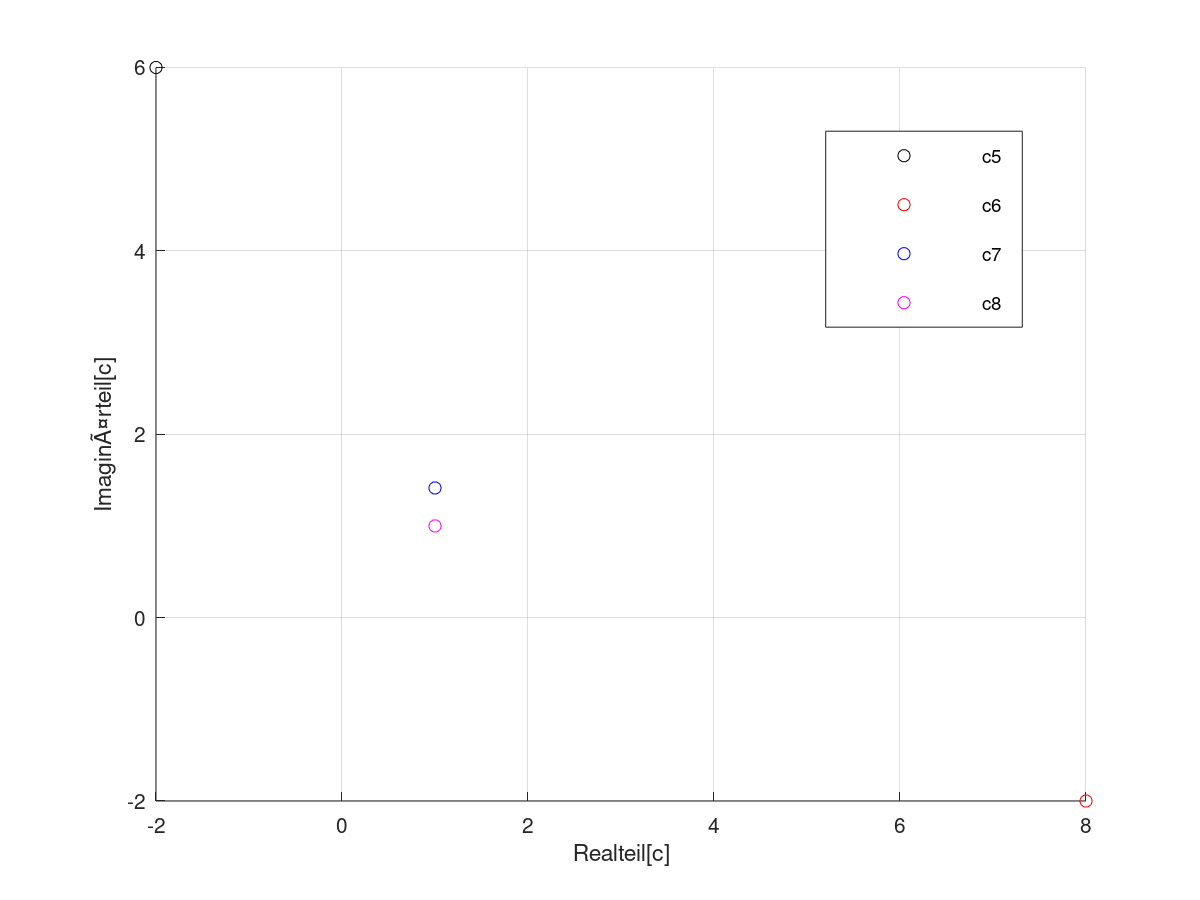
\includegraphics{Aufgabe2_1_b.png}
       }
       \item Siehe dsv2\_1.m
       
       ~
        \hspace{-3cm}
        \scalebox{0.5}{
        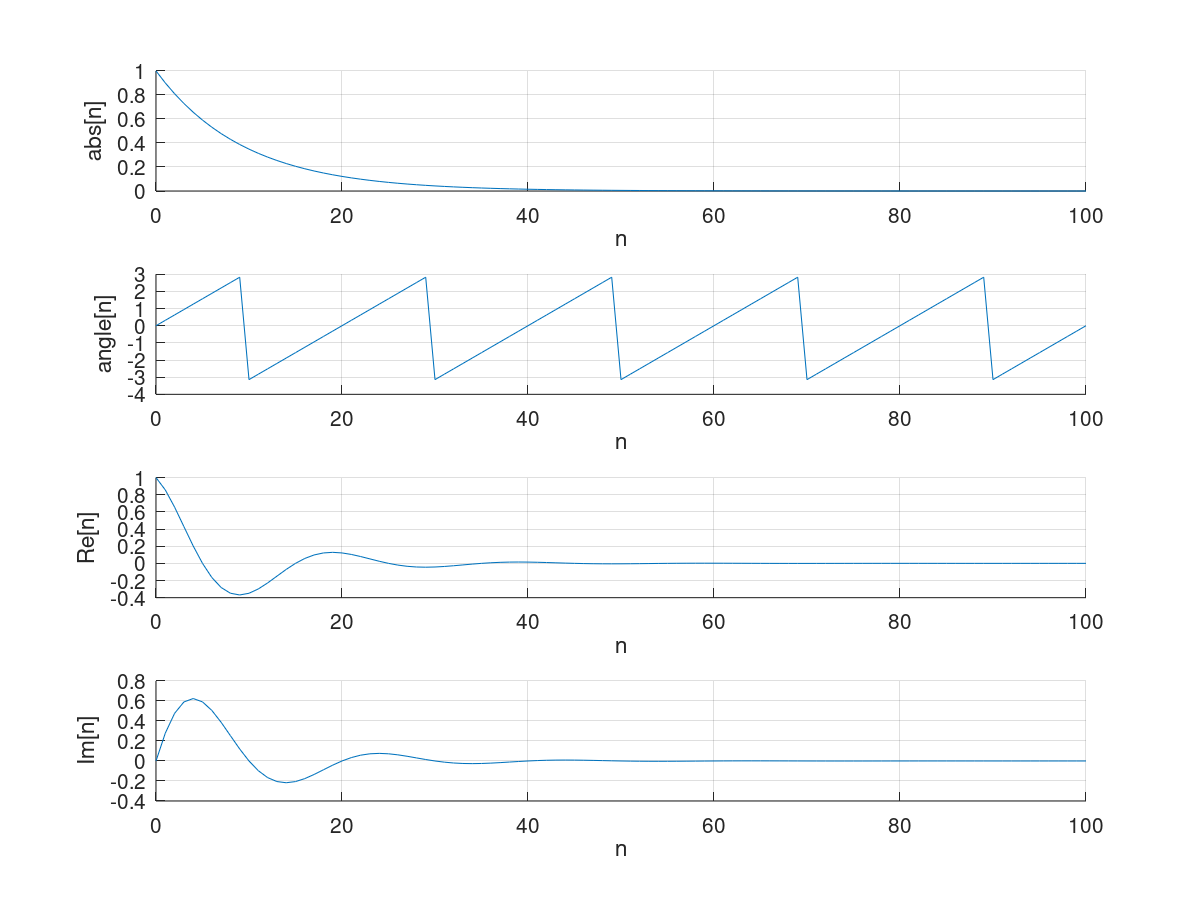
\includegraphics{Aufgabe2_1_c.png}
        }
       \item \begin{align*}
        \alpha_1 &= 45\circ = \frac{45*\pi}{180} = \frac{\pi}{4}= 0,7854 rad \\
        \alpha_2 &= -90\circ = \frac{-90*\pi}{180} = \frac{-1\pi}{2} rad = -1,571 rad \\
        \alpha_3 &= \frac{\pi}{4} = \frac{180^\circ\pi}{4} = 45^\circ\\
        \alpha_4 &= \frac{7\pi}{3} = \frac{\frac{7\pi}{3}*180^\circ}{\pi} = \frac{7 * 180}{3} = 420^\circ
       \end{align*}
    \end{enumerate}
\end{aufgabe}

\pagebreak
\begin{aufgabe}{}

\begin{enumerate}
  \item{}
~

\hspace{-1.5cm}
\scalebox{0.9}{
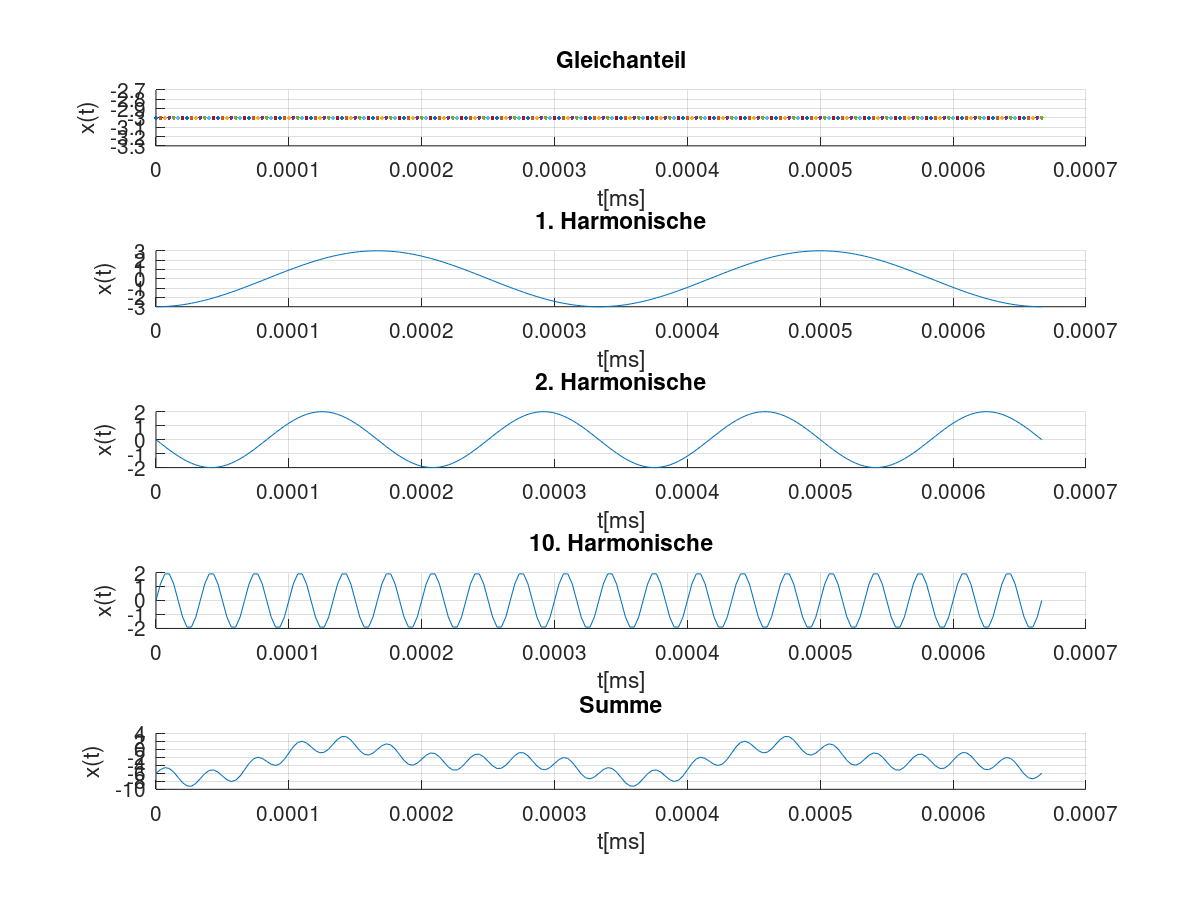
\includegraphics{Aufgabe2_2_a.png}
}
\item Die Koeffizienten $a_k$ und $b_k$ skalieren die Kosinus ($a_k$) bzw. die Sinusanteile der k-ten Harmonischen Schwingung einer durch eine Fourierreihe dargestellten Schwingung.

        Die Koeffizienten sind in der gegebenen Gleichung ablesbar. Die Gleichung hat die allgemeine Form:

        \begin{align*}
            x(t) = \frac{a_0}{2} + a_{k_1}*\cos(2\pi k_1 f_0 t) + a_{k2}*\cos(2\pi k_2 f_0 t) +b_{k3}*\sin(2\pi k_3 f_0 t) ...
        \end{align*}

        Wir können also anhand des ganzzahligen Faktors im Argument des Kosinus das $k$ auf das sich der jeweilige Faktor $a_k$ bezieht, feststellen, indem wir mit 2 dividieren da $2\pi$ ja erhalten bleiben muss. Bei den Sinustermen erhält man entsprechend $b_k$. 

        Die so festgestelleten Faktoren lauten demnach :

        \begin{align*}
            a_0 &= -6 \\
            a_1 &= -3 \\
            b_2 &= -2 \\
            b_{10} &= 2
        \end{align*}

\item
        Die komplexe Form der Fourierreihe ist auch hier endlich und wir können die einzelnen Faktoren der Reihe mit den Formeln :

        \begin{align*}
            c_0 &= \frac{a_0}{2} \\
            c_k &= \frac{a_k -i* b_k}{2}\\
            c_{-k} &= \frac{a_k +i* b_k}{2}
        \end{align*}

        feststellen. Bei fehlendem $a_k$ zu einem vorhandenen $b_k$ muss der fehlende Faktor 0 sein damit der Term in der endlichen Darstellung der Fourierreihe wegfällt et vice versa.
         Zudem muss es zu jedem festgestelltem Koeffizientenpaar $a_k / b_k$, Werte bei $-k$ sowie $k$ geben da die komplexe Fourierreihe ja von $-\infty$ nach $\infty$ läuft, während die Sinus/Kosinus Darstellung von $1$ nach $\infty$, plus den Sonderfall bei $0$, läuft.

        Die errechneten komplexen Fourierkoeffizienten lauten :

        \begin{align*}
            c_0 &= -3\\
            c_1 &= -1.5\\
            c_{-1} &= -1.5\\
            c_2 &= i\\
            c_{-2} &= -i\\
            c_{10} &= -i\\
            c_{-10} &= i
        \end{align*}

        Die komplexe Form der gegebenen Fourierreihe ist somit :

        \begin{math}
          x(t) = -3e^{0} - 1.5e^{2\pi i f_0 t} - 1.5e^{-2\pi i f_0 t} + i e^{4\pi i f_0 t} - i e^{-4\pi i f_0 t} - i e^{20\pi i f_0 t} + i e^{-20\pi i f_0 t}
        \end{math}

        Visualisiert nach den Vorgaben der Angabe ergibt sich folgendes Bild :

        \hspace{-3cm}
        \scalebox{0.5}{
        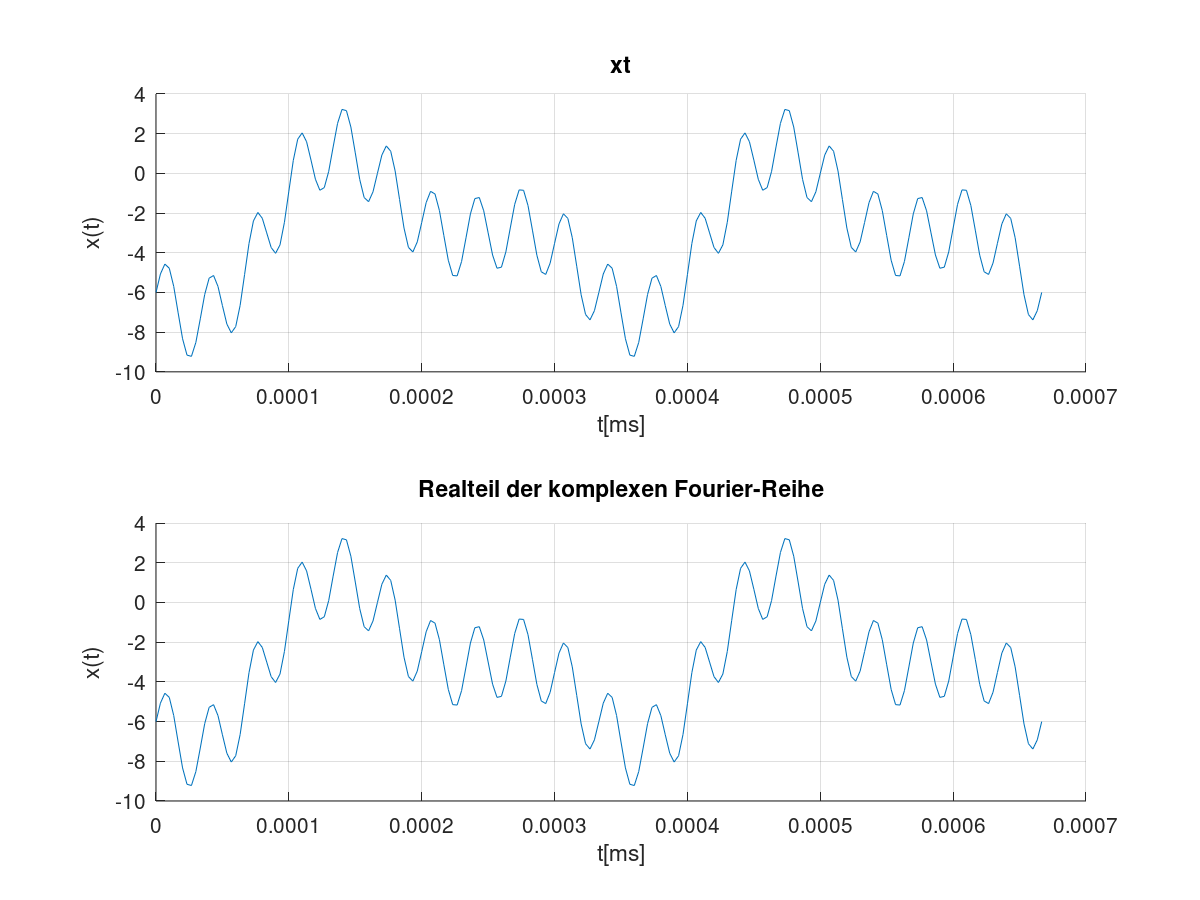
\includegraphics{Aufgabe2_2_c.png}
        }
\item
        Die Frequenz hat keinen Einfluss auf $a_k$ und $b_k$ und somit auch keine Einfluss auf die entsprechenden $c_k / c_{-k}$.
\end{enumerate}
\end{aufgabe}
\begin{aufgabe}{}
  \begin{enumerate}
    \item LTI ist ein Akronym aus dem Englischen und bezeichnet ein \textit{linear time-invariant} system also zu Deutsch ein lineares zeitinvariantes System.
    

          Linear ist ein System dann wenn eine Summe von beliebig vielen Einganssignalen zu einer proportionalen Antwort des Ausgangsignales führt. Die System muss also dem Überlagerungsprinzip folgen.

          Zeitinvarianz bezeichnet eine Eigenschaft des Systems die besagt dass wenn ein Eingangssignal zeitverschoben erscheint, das Ausgangssignal sich nur um diese Zeitverschiebung unterscheidet. Das System reagiert also zu jedem Zeitpunkt mit der gleichen Antwort.
  
  
    \end{enumerate}
\end{aufgabe}
\pagebreak
\begin{aufgabe}
    ~

    \hspace{-1.5cm}
    \scalebox{0.6}{
    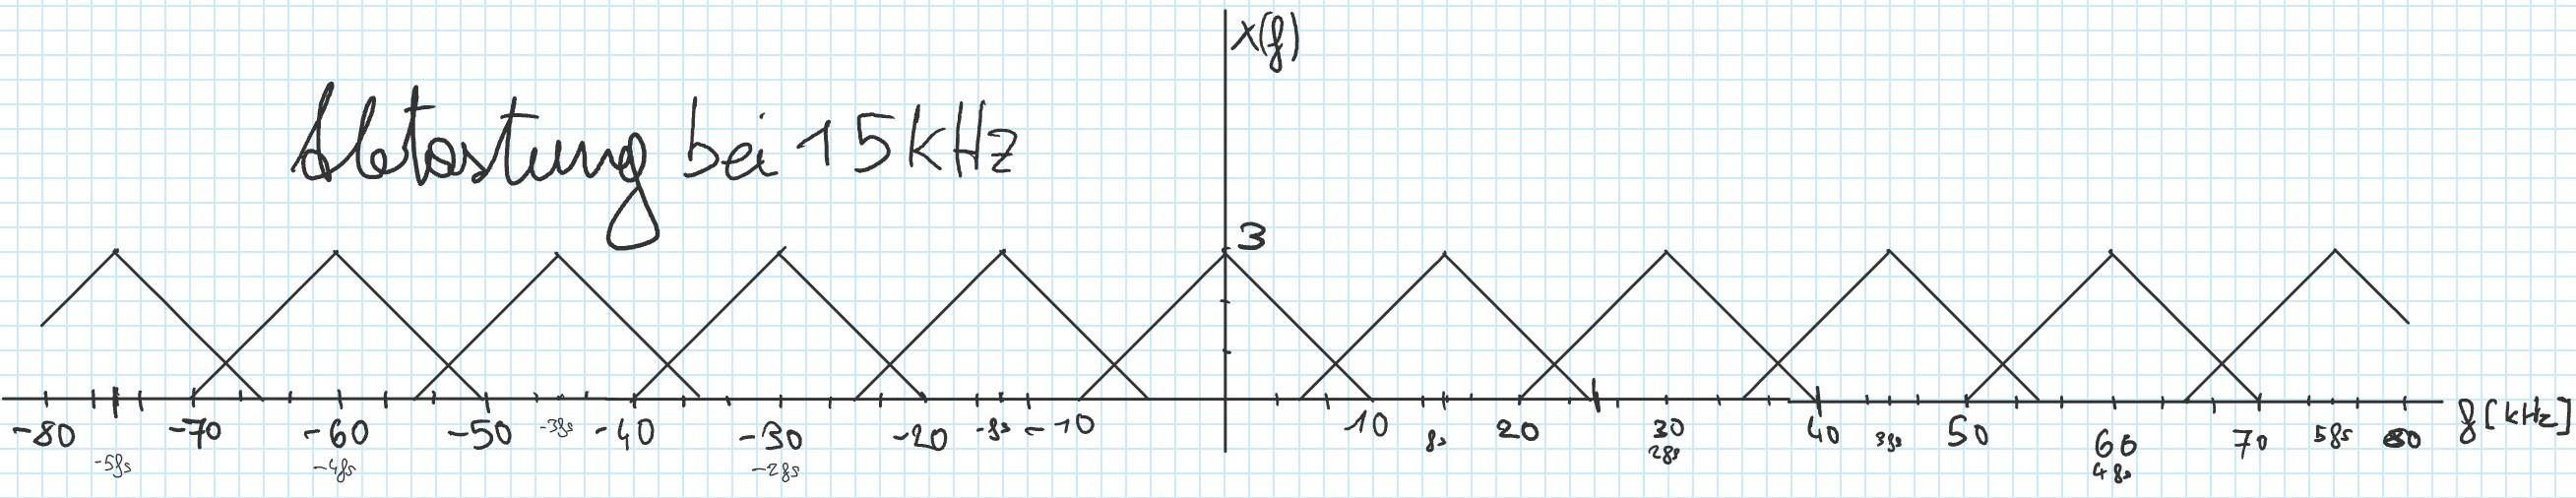
\includegraphics{Abtastung15khz.jpg}}

    Bei einer Abtastung mit 15kHz sieht man deutlich die Überlagerungen der Spektren. Durch eine Aufsummierung der Signale im Überlagerunsbereich erhält man folgendes Spektrum :

    \hspace{-1.5cm}
    \scalebox{0.6}{
    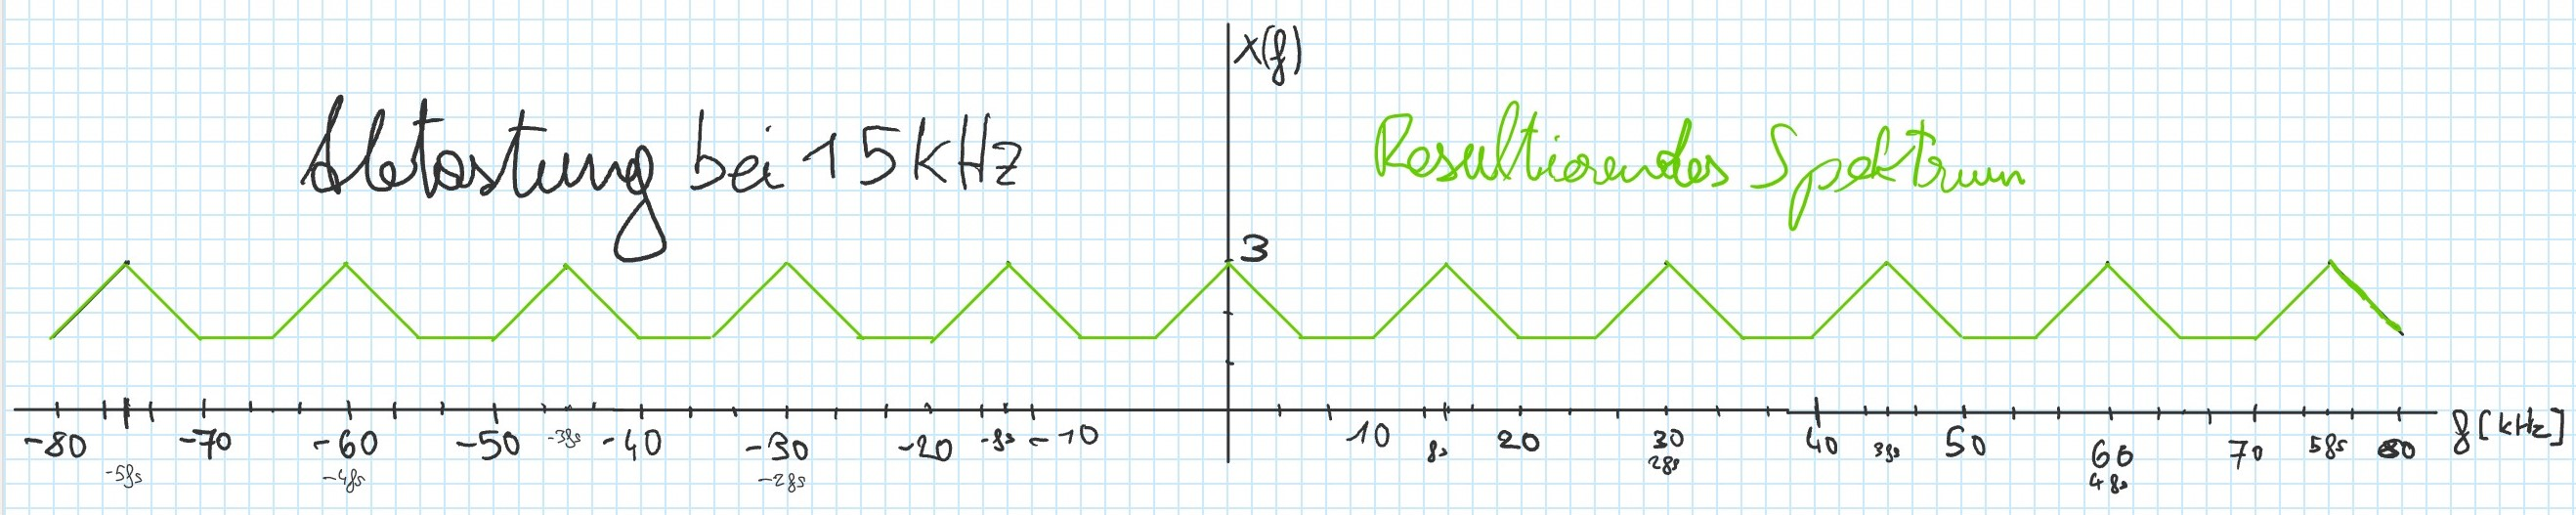
\includegraphics{Abtastung15khzResult.jpg}}


    ~

  Bei einer Abtastung mit 25kHz kommt es zu keinen Überlagerungen :

    ~

    \hspace{-1.5cm}
    \scalebox{0.6}{
    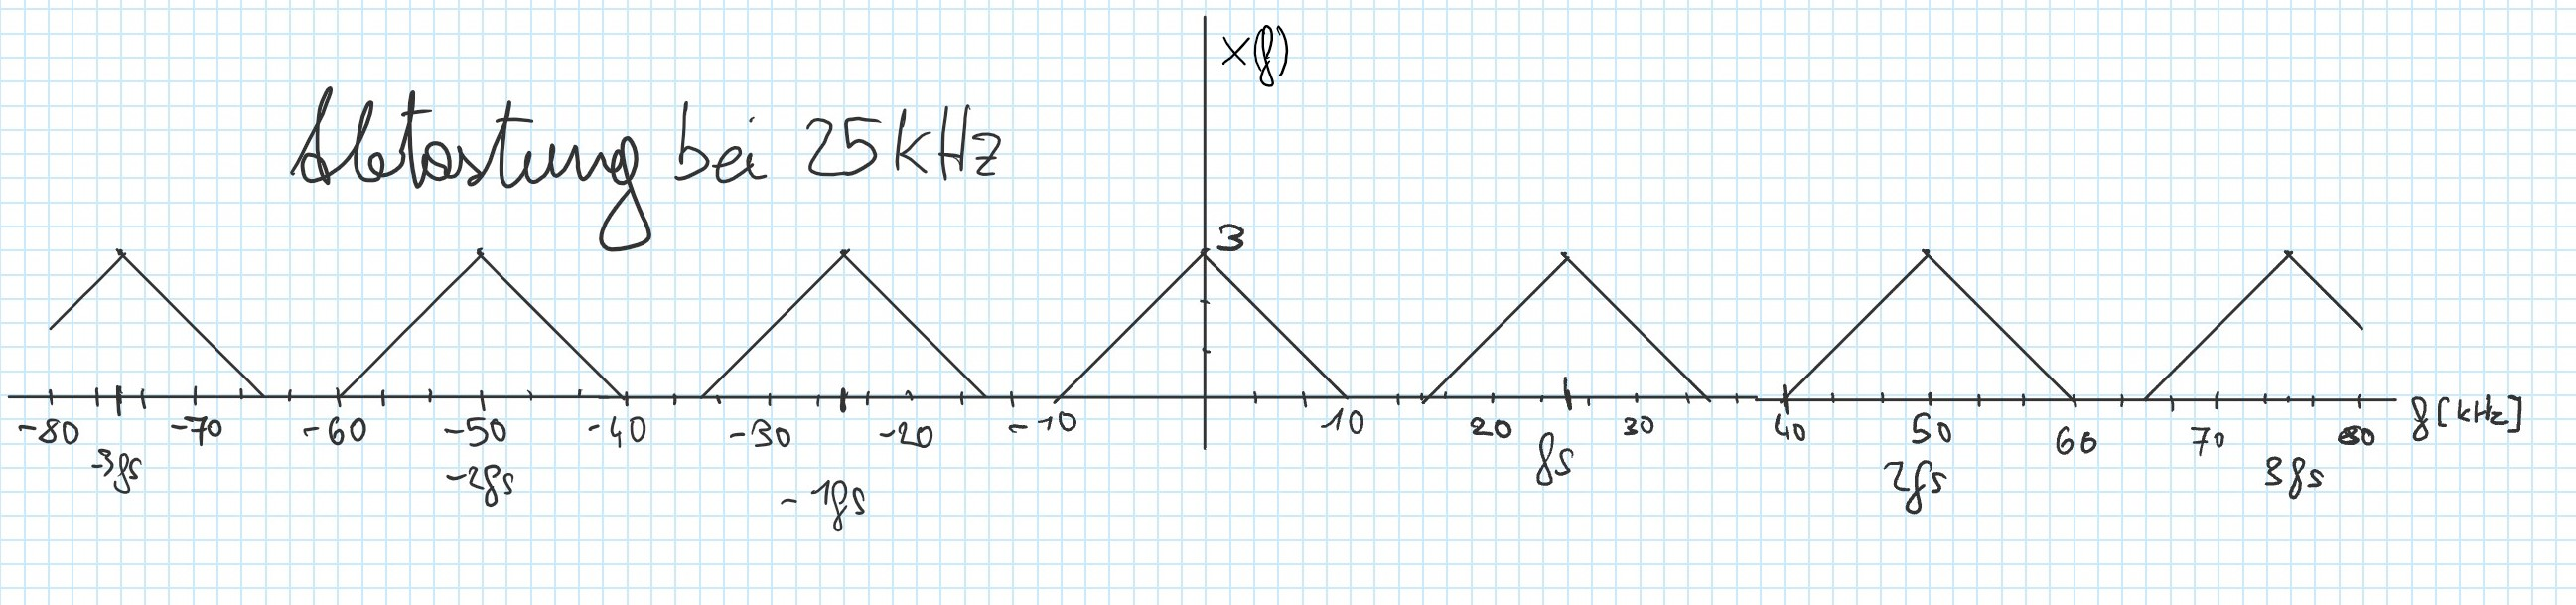
\includegraphics{Abtastung25khz.jpg}}

    Um ein Analogsignal verlustfrei wieder rekonstruieren zu können muss man nach dem Nyquist-Shannon-Abtasttheorem mit einer Frequenz $f_s$ von $f_s >= 2*f_{max}$ abgetastet werden. Wie man an dem Beispiel mit $f_s = 15kHz$ sehen kann geht bei einer zu niedrigen Abtastfrequenz Information über das Spektrum des abgetasteten Signals verloren und es entsteht Aliasing. Um die höherfrequenten Resonanzen, die Wiederholungen des Signals, zu vermeiden werden die Signale auch bandbegrenzt.
\end{aufgabe}
\end{document}
